
\chapter{Background and Related Work}

This chapter will establish the foundation of Persuasive recommendation system along with active learning and critiquing approach. Prior to in depth analysis, it will provide important background information along with some required definitions. Additionally, related work will presented, as the chapter proceed further to the end..\newline

\section{Definitions}

\subsection{Recommender System}

Recommender Systems (RS) are search tools, which supports user decision-making by providing the suggestion that, are according to their interests. Such systems are widely uses from social networking through e-commerce sites in order to achieve different purposed. In e-commerce site, they help not only to serve the customer by suggesting items according to their preferences but also support business to improve in its sale. On the other hand in social network site, to suggest friends or pages like according to user preferences. According to Ricci [Ricci, 2010] "RS are information search tools that have been recently proposed to cope with the "information overload" problem, i.e., the typical state of a web user, of having too much information to make a decision". Proposed solution [Resnick and Varian, 1997] is an intelligent system that suggests the product or service that fulfill the user’s preference in given context or situation. Suggestions provided by such systems are depended on the model how they are keeping information. Majority of RS are typically community based. In this kind of modeling suggestions are depend about item popularity among the user. Where popularity is calculated by ratings. Important question that arise in such systems are to find item accuracy according user preferences. On the other hand Personalized models are used that depends on the various factors which includes user’s preferences, history of bought/liked items, or the items the user has ranked in the past. Various techniques are use in the developing of recommender system. Classification of recommendation systems [Ricci, 2001] will be discussed as follows.

\subsubsection{Content-based filtering}

In this technique recommendations are based on user preference. System recommend items that similar to one is liked by user. Item similarity is calculated by features associated with the compared items [Ricci , 2001]. For example, if a user has rated positively recipe A under the category of sweet then next suggestion that is provided by the system is one which is similar to one user has like before.

\subsubsection{Collaborative-based}

Collaborative filtering is technique in which system find the correlation between item and user based opinions of other users which having a similar taste in past [Shapira , 2001]. Initially system calculates all similar taste users for the current user and calculate the recommended item that contains either rated or liked by other users having similar taste. Importantly in this approach item speciation will not be considered. For instance, if user like recipe A then next recommendation would be recipe that there are other users who liked recipe A also liked recipe B.

\subsubsection{Demographic}

Recommendations are generated according to user demographic profile. Recommendations can be produced for different demographic niches by combining the ratings of users in demographic clusters [Mahmood, 2007]. For example, suggestion provided by the systems are shown according to user’s age. 

\subsubsection{Knowledge-based}

In knowledge-based systems item recommendation is based on domain specific knowledge, which justifies how certain item features meet according to user’s preferences [Ricci , 2001]. Importantly, it uses predication techniques namely Case-based reasoning which reuses the cases past cases that are similar to current case in order to identify item set of recommendation.

\subsubsection{Community-based}

Type of recommendations provided by this kind of system based on preference of user friends. According to Ricci research [Ricci, 2001], People tend to rely more on recommendations provided by friends rather than on recommendations from anonymous individual having similar taste. Such type of RS model relies on user’s social relations including preference of user’s friends. Suggestions depend on rating that is provided by user’s friends.

\subsubsection{Hybrid Recommender Systems}

Hybrid system is a fusion of any two or more techniques motioned above. Ricci [Ricci , 2001] explains the motivation behind such system to avoid the limitation of one technique. For instance, Collaborative filtering have cold startup problem i.e. they are unable to suggest those items, which have no ratings. On the other hand Content-based doesn’t have such limitation by combination of both approach new hybrid system can be formed. Similarly, Burke [Burke, 2007] proposed the combination techniques to create a new hybrid system.

\subsection{Contexts}
Recommendation techniques used by traditional system relies on vector of item rating and user preferences. According to Suchman \cite[Suchman, 1996]{suchman1986plans} these approaches ignores the notion of “situated actions”,which infers that user have particular context and item preference within one context may be different for another context\cite[Adomavicius, 2011]{adomavicius2011context}.
Absence of context may lose information predictive power because of aggregation of multiple contexts. For instance, User wants to buy cloths of his child gives results according to his dressing choice due to contextual information missing.\newline

Since context is a multi dimension topic therefore vast amount of research has been done in area, narrowing down role of context in recommender system, context can be defined as all information according to given situation. One of the early definitions of context in terms of operation \cite[Schilit, 1994]{schilit1994disseminating} defined as where you are, who you are with, and what resources are nearby.  As reach goes by new and most sited definition of context according to Adomavicius \cite[Adomavicius, 2011]{adomavicius2011context} “Any information  that  can  be  used  to characterize  the  situation  of  an entity.  An entity is a person, place, or object that is considered relevant to the interaction between a user and an application, including the user and applications  themselves”. Futhermore, \cite[Dourish, 2004]{dourish2004we} while observing the uses of context he classified into to two views namely \textit{ representation } and \textit{ interaction } views.  He assumed four key assumptions for describing representational view. context is independent from underlying activity, delineable, stable and in a form of information. According to this view, context can be known prior as it is a set of observable attributes and structure of these attributes does not change with respect to  time. Futhermore, \cite[Dourish, 2004]{dourish2004we} while observing the uses of context he classify into to two views namely \textit{ representation } and \textit{ interaction } views.  He assumes four key assumptions for describing representational view context is independent from underlying activity, delineable, stable and in a form of information. According to this view, context can be known prior as it is a set of observable attributes and structure of these attributes does not change with respect to time. On the other hand interactional view features are dynamic. It assumes that context and activity have a relationship.\newline

Adomavicius \cite[Adomavicius, 2011]{adomavicius2011context} put forward research \cite[Dourish, 2004]{dourish2004we} on categories  and  explains recommender system can have different types of knowledge, which may include the exact list of all the relevant factors, their structure, and their values, about the contextual factors. He classifies the knowledge of a recommender system about the contextual factors into three categories; \newline

\textit{Fully observable} refers to explicit knowledge of structure and values of contextual factors of application at the time when recommendation are made. Theses factors refer as Purchasing Purpose, Shopping Companion and time. For example, User wants to buy shirt, besides having information of selling point and item. Theses may include information about the time, for whom. \textit{Partially observable} application has some of information about the context explicitly. For instances, Purchasing Purpose, Shopping Companion and time all information given but the structure is missing.\textit{Unobservable} no information regarding contextual information is provided explicitly. Utilizing only the latent knowledge of context in an implicit manner makes recommendations. For example, the recommender system may build a latent predictive model, such as hierarchical linear or hidden Markov models, to estimate unknown ratings, where unobservable context is modeled using latent variables.\newline

Furthermore, Adomavicius \cite[Adomavicius, 2011]{adomavicius2011context} find out the dependency of contextual factors over time and classify them into categories. \textit{Static} The relevant contextual factors and their structure remains the same (stable) over time. \textit{Dynamic} contextual factors change in some way.

\begin{figure}[h]
	\centering
	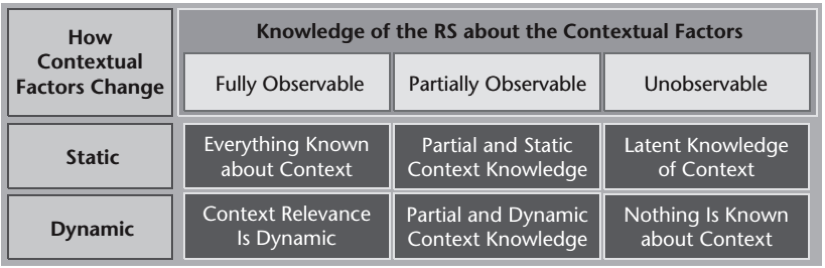
\includegraphics[width=.98\linewidth]{figures/ch2_context_dimensions.png}
	\caption{Contextual Information Dimensions.} 
	\cite[Adomavicius, 2011]{adomavicius2011context}
	\label{fig:ch2_context_dimensions}
\end{figure}

\subsubsection{Representing and Modeling Context}

Classical the recommendation system has the prediction problem in which user’s rating for item reflects the degree of user preferences. Therefore, a recommender sys- tem tries to estimate a rating function.

\begin{equation} 
R : Users x Items \rightarrow Ratings
\end{equation}

It’s a 2D matrix of user-item to an ordered set of rating values. Where R a general-purpose\textit{utility} (or preference).Since the value of R is partial function therefore rating of all user-item are not known which arise the predication problem.

\begin{equation} 
R : Users x Items x Contexts \rightarrow Ratings
\end{equation}

In contrast, context aware recommend have additional evidence to estimate user preference on unseen item. Contextual evidence can be applies to input function and viewed as “multidimensional”. Where, any information related to data and user can be refer as Contextual information

\subsubsection{Paradigms for Using Contextual Information}

According on algorithm approaches of context aware recommendation, represents in form of \textit{U x I x C x R}, Where U is for User, R denotes rating, C is contextual dimension, and produce contextual recommendations list i1, i2, i3 ... for each user u. Figure \ref{fig:ch2_context_recommender_system_paradigms} illustrates the Paradigms used in processing Contextual Information. These are categories as follows:\newline

\textit{Contextual prefiltering} In this filtering Context is applied an input. With the help of any classical 2D recommendation data selection approach, applies current context which is used for selection of relevant ratings and dataset.\newline

\textit{Contextual postfiltering} Prediction of rating is applied with the help of traditional 2D recommender system technique. On the resultant set of recommendation applies the context for each user. \newline

\textit{Contextual modeling} directly integrates the contextual information in the modeling technique as part of the rating estimation. .\newline


\begin{figure}[h]
	\centering
	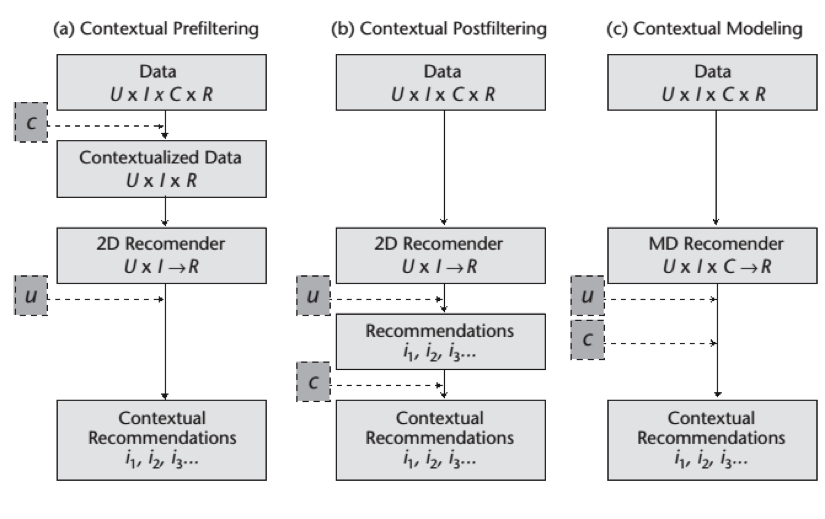
\includegraphics[width=1\linewidth]{figures/ch2_context_recommender_system_paradigms.png}
	\caption{Paradigms for Incorporating Context in Recommender Systems.}
	\cite[Adomavicius, 2011]{adomavicius2011context}
	\label{fig:ch2_context_recommender_system_paradigms}
\end{figure}


\subsection{User Profiling}

User profiling is process of acquiring information about the user, which helps in constructing the user model. Rate of acceptance and effectiveness of recommendation will effect how much system has information about the user. Tang \cite[Tang, 2010]{tang2010combination} explains as  In the context of software applications, a user profile or user model comprehends essential information about the user. It also refers and digital representation of person in a system and hold the person’s preferences. Variations in user profile content depend on application. Some applications depend on demographic information of user while other relies on rating, liking, disliking or other preferences. Also, consideration of user interaction and behavior take plays an important role for providing precise recommendations.\newline

Schiaffino \cite[Schiaffino, 2009]{schiaffino2009intelligent} stated that discovery of differences and similarities in interests among users is a key to provide personalized recommendations  Which implies that application users have different preferences and interests to achieve their goals which leads to importance of creation of user profile in order to find out relationship between user according to their interests. Content of user profile depends on application domain and variations are presents application. Categorically there are two methods to gather content of user profile. First method is manually, in this technique users are being interviewed, fill the some form or questionnaires. For instance asking about his demographic profile like where he is form, which dishes he likes or rating based questions like how frequently he eats junk food? On the other hand by mean of implicit learning about user preference which requires artificial intelligence (AI) techniques like Case-based reasoning, Bayesian Networks, Artificial neural networks. Most of these techniques are beyond the scope of this work so they will not be described in more details. Fundamentally there are two different alternatives to build a user profile; either the information is obtained explicitly from user or implicitly through the observation of user’s actions. The next section describes these alternatives.\newline

\subsubsection{Explicit Profiling}

Explicit profiling often known as explicit user feedback is the simplest way of gathering information about users. In this technique, user has to fill questioners in order to develop profiles. Profiles developed by this techniques are totally depends on the questioner. Normally, data contains demographic information regarding the user like name, age, location and other preferences. Gauch \cite[Gauch, 2007]{schiaffino2009intelligent} suggests input methods that allows user to rate item according to their interest. Alternatively system can provide check box and text field in order to get preference of user. \textit{HTML forms, Questionnaires, Rating, User preference and Touch sensors} are some techniques  user to obtain explicit profile. Where as, the limitation of this technique is that it requires user time and willingness to provide their data.  Some user has reservation in regards to provide their personal information because of potential privacy concern. However user’s preference can always be determine via this technique.\newline

\subsubsection{Implict Profiling}

Implicit profiling is also known, as implicit user feedback is another approach for building user profile. It is popular and widely used methodology to develop user profile based on user ‘s acquired information. Mostly profiles are derived form monitoring or observing user activities.  Information acquires by the system helps them to ensure the given recommendation is according to user interest. For example popular website for watching video YouTube. It recommendation is made on similar to those video is watch by user in past.  Single-sign-on (SSO) \cite{ hursti1997single } one the most common methodology for user registration. Since the information is implicit they may contains user demographic information. Similarly user preference like, dislike, location can be fetch by integrated related third party services. Information obtain form this mechanism plays an important role in personalized recommendation system. \ textit{Search logs, Browser cache and User monitoring agents} are some techniques used to generate implicit profile. Main advantage of this technique user doesn’t have to enter form and provide their information. Kelly \cite[Kelly, 2003]{schiaffino2009intelligent} provides an overview of standard techniques that are help to build user profile and information types about the user that can be in inferred from user’s behavior.\newline

\subsection{Conversation-based Critiquing Recommenders}

Recommender systems may also vary in the function to the extent that user can get engage in the dialogues. In traditional techniques data was collect once and terminate after recommendation are made. Assumption of these approaches is user know all his preferences at the beginning which was not the case. Whereas, user taste may change over time and he want to interact with different option. Smyth \cite[Smyth, 2003]{ mcginty2003role} handles this problem and called “Conversational recommendation system” (CRS). He states that CRS have their origins in conversational case-based reasoning (CCBR) which apply similar techniques to elicit query information in problem solving domains and diagnostic tasks.” It is an interactive approach in which user preferences are establish through conversation session. At first initial set of recommendations are given to the user. System adapts the user feedback to further enhance the recommendations. Smyth \cite[Smyth, 2003]{ mcginty2003role} distributed feedback into three categories.\textit{ Rating-based} in this approach user provides rating for an specific item.\textit{ Critique-based} where user add constrain over item features.\textit{ Preference-based } in which user indicates its preference for one particular item over the others.\newline

\subsection{Active Learning}

Active learning (AL) is a methodology to learn about user’s preference by asking him/her to rate a number of item knows as training point \cite[Rubens, 2011]{ rubens2011active}. Data is formed by model that approximates user’s preference. It is useful where user’s preferences are change with respect to context.  Rashid \cite[Rashid, 2008]{rashid2008learning} explains that objective of AL may varies according to objectives of recommendation systems.  For example, what is important in the recommender system being built? The difficulty of signing-up (user effort)? If the user is happy with the service (user satisfaction)? How well the system can predict a user’s preferences (accuracy)? Furthermore, this approach can solve cold startup problem in an effective manner. Figure \ref{fig:ch2_active_learning} explains how interactive process works in order to obtain training data, unlike passive learning, where data is simply given to system in a linear fashion. Rubens \cite[Rubens, 2011]{ rubens2011active} categorized AL method according to their primary goal.  

\begin{figure}[h]
	\centering
	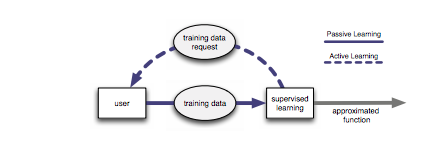
\includegraphics[width=1\linewidth]{figures/ch2_active_learning.png}
	\caption{Active vs Passive Learning}
	\cite[Rubens, 2011]{ rubens2011active}
	\label{fig:ch2_active_learning}
\end{figure}

\subsubsection{Instance-based Methods}

In kind of approach points selection is relies on their properties in an attempt to predict user’s rating by the closet match to other user, without have explicit knowledge about underlying model \cite[Adomavicius, 2005]{adomavicius2005toward}. Whereas, it assumes that under consider model any data and rating predictions are accessible.

\subsubsection{Model-based Methods}

In this methodology point selection is based on best construct model that explains data supplied by the user to predict user ratings \cite[Adomavicius, 2005]{adomavicius2005toward}. Similarly, select point are used to maximize the reduction of expected error of the model. Whereas, it assumes that in addition to any data available to instance-based methods, the model and its parameters are also available. 

\subsubsection{Modes of Active Learning: Batch and Sequential}

Since the expectation of user is to high for the system while they are performing interaction. They expect immediate output from the system. One common approach is to recalculate the rating of item once user rated single item, known as sequential mode. However another possibility is that to allow user to rate several features of items or rate several item before model readjustment known as batch mode. As immediate reflection of data in sequential mode is an advantage but cost of interaction will always effect. Therefore, trade-off exists between Batch and Sequential AL: the usefulness of the data vs. the number of interactions with the user 

\subsection{Persuasive Recommedations}

\section{Related Work}

\subsection{User's Food Preference Extraction for Personalised Cooking Recipe Recommendation}

\subsection{Knowledge Base Framework for Development of Personalised Food Recommendation System}

\subsection{Interactive Explanations in Mobile Shopping Recommender Systems}

\subsection{Active Learning Strategies for Exploratory Mobile Recommender Systems Interactive Explanations in Mobile Shopping Recommender Systems}